
Second-level tiling allows us to improve data locality significantly. Now, we can rely on the vectorization process to improve CPU resource utilization and reduce L1 bandwidth by a factor of SIMD width. However, further optimization is required to reduce the L1 bandwidth and achieve maximum CPU utilization. So, we apply the register-blocking/tiling (\textbf{RT}), where we compute a patch (third-level tile) of the second-level tile that fits in the vector register. Elements from the input matrices are loaded into the memory and used multiple times to update the patch, effectively reducing the memory accesses for the input and output.

\begin{figure}[htbp]
\centerline{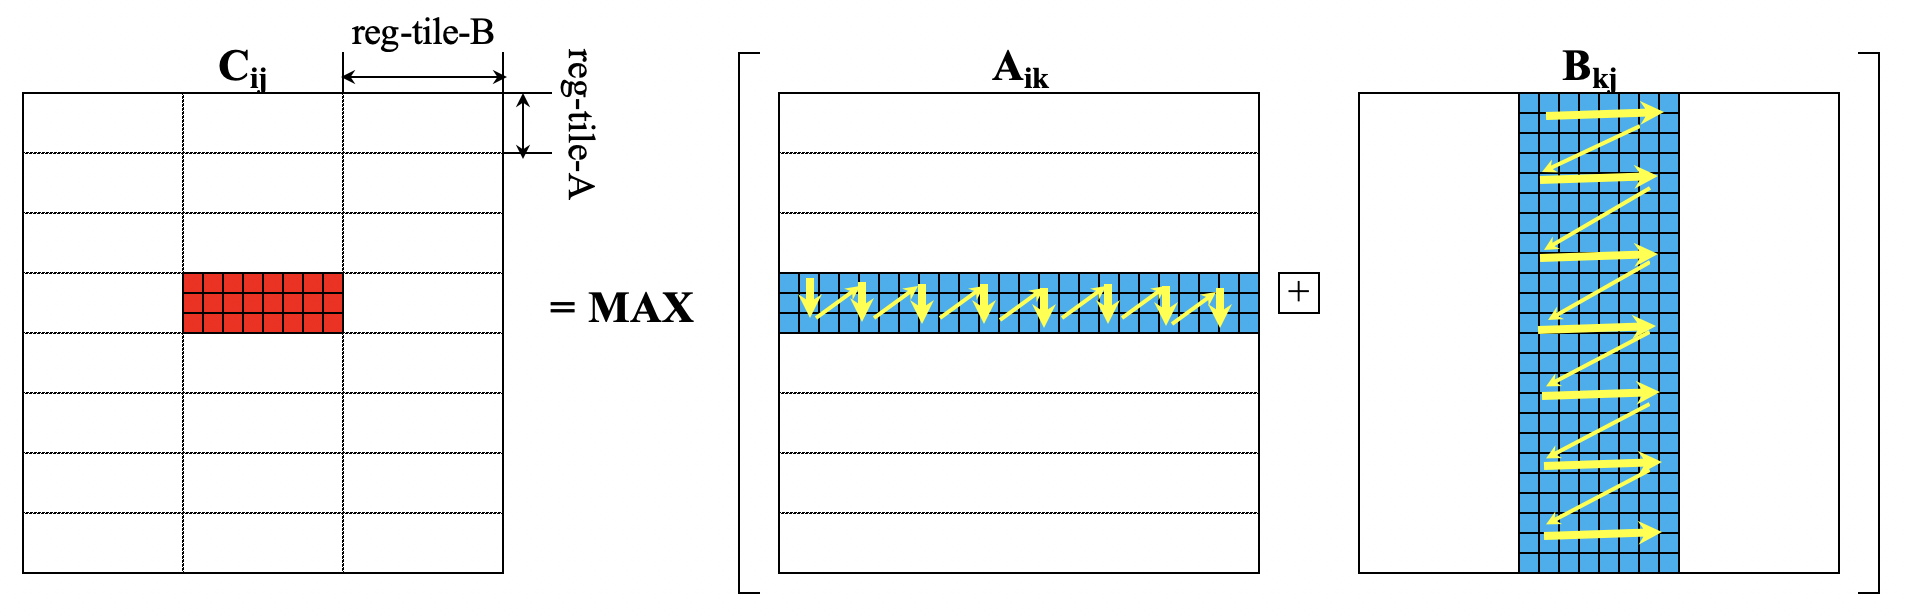
\includegraphics[scale=0.25, trim=5 5 5 5,clip]{content/figures/register_tile.png}}
\caption{Register Tiling (\textbf{RT})}
\label{fig:regiser_tile}
\end{figure}

Sequential memory access is a well-known property of any modern CPU-specific register-tiled kernel. Its performance depends on how the scalar and vector inputs are read from the memory and their alignments. So, we transform the first input matrix (let us call this A) and the second input matrix (let us call this B) such that the memory access pattern from the register-tile kernel is sequential. Figure~\ref{fig:regiser_tile} shows the memory access pattern of our register tile. Previously, similar techniques were also implemented for a register tile that performed FMA operations by Huang et al. \cite{FLAWN80}. We observe that an inner-$F$-table triangle or $S_{2}$ can be used several times as a $A$ or $B$ operand. Thus, it is possible to transform each triangle with two different memory layouts once and avoid transforming the same tile multiple times. 

\subsubsection{Buffer Transformation Strategy}
We have explored three buffer transformation techniques for accessing data sequentially within the register-tiled code. They are based on when we transform \textbf{register-tile-operand-A} and \textbf{register-tile-operand-format-B}. The first one \textbf{ [MPT+RT]:v1} transforms each inner $F$-table and $S_{2}$ to \textbf{register-tile-operand-A} and \textbf{register-tile-operand-format-B} exactly once but  introduces four new $F$-table variables - $F(A)$,  $F(B)$, $S_{2}(A)$, $S_{2}(B)$ in the system. The inner reductions $R_{1}$ and $R_{2}$ also use $S_{2}$ as the other operand for the max-plus operation. \textbf{ [MPT+RT]:v2} uses on-the-fly transformation for both of the operands, and \textbf{[MPT+RT]:v3} uses pre-transformed $S_{2}$ but transforms the inner $F$-table on the fly. 




